\documentclass[11pt,letterpaper]{article}

% =====================================================================
%  Two-Layer MCP Architecture: From Tool Server to Agent Platform
%  A position paper for NOAA/EMC leadership and computational
%  meteorologists
% =====================================================================

\usepackage[margin=1in,top=1in,bottom=1in]{geometry}
\usepackage[T1]{fontenc}
\usepackage[utf8]{inputenc}
\usepackage{lmodern}
\usepackage{microtype}
\usepackage{xcolor}
\usepackage{graphicx}
\usepackage{booktabs}
\usepackage{tabularx}
\usepackage{enumitem}
\usepackage{titlesec}
\usepackage{fancyhdr}
\usepackage{hyperref}
\usepackage{mdframed}
\usepackage{tcolorbox}
\tcbuselibrary{skins,breakable}
\usepackage{tikz}
\usetikzlibrary{shapes.geometric,arrows.meta,positioning,fit,backgrounds,calc,shadows.blur,patterns}
\usepackage{pgfplots}
\pgfplotsset{compat=1.17}

% ---------- Palette (NOAA-friendly blues and neutrals) --------------
\definecolor{noaablue}{HTML}{1F3A5F}
\definecolor{accent}{HTML}{2B6CB0}
\definecolor{accentlight}{HTML}{BEE3F8}
\definecolor{emcgold}{HTML}{B7791F}
\definecolor{warm}{HTML}{C05621}
\definecolor{ok}{HTML}{2F855A}
\definecolor{ink}{HTML}{1A202C}
\definecolor{paper}{HTML}{F7FAFC}
\definecolor{subtle}{HTML}{718096}
\definecolor{layer1}{HTML}{2C5282}
\definecolor{layer2a}{HTML}{3182CE}
\definecolor{layer2b}{HTML}{2F855A}
\definecolor{layer2c}{HTML}{975A16}

% ---------- Typography -----------------------------------------------
\titleformat{\section}
  {\normalfont\Large\bfseries\color{noaablue}}{\thesection}{0.7em}{}
\titleformat{\subsection}
  {\normalfont\large\bfseries\color{accent}}{\thesubsection}{0.7em}{}
\titleformat{\subsubsection}
  {\normalfont\normalsize\bfseries\color{ink}}{\thesubsubsection}{0.6em}{}

% ---------- Page headers ---------------------------------------------
\pagestyle{fancy}
\fancyhf{}
\fancyhead[L]{\footnotesize\color{subtle} MDC MCP RAG}
\fancyhead[R]{\footnotesize\color{subtle} Two-Layer MCP Architecture}
\fancyfoot[C]{\thepage}
\renewcommand{\headrulewidth}{0.2pt}
\renewcommand{\footrulewidth}{0pt}

% ---------- Links ----------------------------------------------------
\hypersetup{
  colorlinks=true,
  linkcolor=accent,
  urlcolor=accent,
  citecolor=accent,
  pdftitle={Two-Layer MCP Architecture: From Tool Server to Agent Platform},
  pdfauthor={MDC MCP RAG Team},
  pdfsubject={AWS Bedrock AgentCore MCP Architecture},
}

% ---------- Callout boxes --------------------------------------------
\newtcolorbox{keyidea}[1][]{
  enhanced, breakable,
  colback=accentlight!30, colframe=accent, coltitle=white,
  fonttitle=\bfseries,
  title={Key idea},
  arc=2pt, boxrule=0.6pt,
  left=8pt, right=8pt, top=6pt, bottom=6pt,
  attach boxed title to top left={xshift=8pt, yshift=-9pt},
  boxed title style={colback=accent, size=small, arc=2pt},
  #1
}

\newtcolorbox{impact}[1][]{
  enhanced, breakable,
  colback=white, colframe=emcgold, coltitle=white,
  fonttitle=\bfseries,
  title={Operational impact},
  arc=2pt, boxrule=0.6pt,
  left=8pt, right=8pt, top=6pt, bottom=6pt,
  attach boxed title to top left={xshift=8pt, yshift=-9pt},
  boxed title style={colback=emcgold, size=small, arc=2pt},
  #1
}

% ---------- Document -------------------------------------------------
\begin{document}

% ============== Cover block ==========================================
\begin{titlepage}
\centering
\vspace*{1.2in}
{\color{noaablue}\Huge\bfseries Two-Layer MCP Architecture\par}
\vspace{0.25in}
{\color{accent}\LARGE From Tool Server to Agent Platform\par}
\vspace{0.6in}

\begin{tcolorbox}[colback=accentlight!30, colframe=accent,
                  width=0.8\linewidth, boxrule=0.4pt, arc=3pt]
\centering
\itshape A position paper for NOAA/EMC leadership and computational\\
meteorologists on the architectural payoff of our\\
AWS Bedrock AgentCore deployment of the MDC MCP RAG Server.
\end{tcolorbox}

\vfill
{\normalsize
MDC (Modeling Development Center)\\
NOAA/NWS/NCEP/EMC\\
\vspace{0.3in}
\color{subtle}
Version 1.0 \quad\textbullet\quad May 7, 2026\par}
\end{titlepage}

% ============== Executive summary ====================================
\section*{Executive summary}
\addcontentsline{toc}{section}{Executive summary}

\begin{mdframed}[linecolor=noaablue, linewidth=0.8pt, backgroundcolor=paper,
                  leftmargin=0pt, rightmargin=0pt, innertopmargin=10pt,
                  innerbottommargin=10pt, innerleftmargin=12pt,
                  innerrightmargin=12pt, roundcorner=3pt]
The MDC MCP RAG Server---a 51-tool knowledge and analysis service for NOAA's
Global Workflow---has been deployed to \emph{AWS Bedrock AgentCore Runtime}.
The immediate benefit is operational: authenticated, multi-user, auto-scaling
access to our graph and vector knowledge bases from anywhere on the public
internet (GitHub, HPC login nodes, analyst laptops), with private VPC
isolation for the data stores themselves.

The \emph{architectural} benefit is more consequential. The deployment
establishes a clean two-layer pattern: a stable, shared \textbf{tool library}
at Layer~1, and a proliferating ecosystem of \textbf{task-specific agents}
at Layer~2. Each agent is a lightweight ($\sim$80 LoC) independently deployed
service that orchestrates our tools into a purpose-built analytical
assistant---for example, an EE2 compliance auditor invoked automatically
when a CI build fails, or a code review assistant invoked on every pull
request.

This paper explains the architecture, shows three concrete agent use cases
that become viable today, and describes the operational, cost, and trust
properties that flow from the two-layer partition.
\end{mdframed}

\vspace{6pt}

\noindent\textbf{Intended audience:} EMC directorate, branch chiefs,
computational meteorologists building or operating Global Workflow, and
anyone evaluating how automated analytical capabilities are being expanded
across our development lifecycle.

\vspace{0.3in}
\tableofcontents
\newpage

% ============== Section 1: What was built ============================
\section{What we built, and what it is not}

The team deployed our MCP (Model Context Protocol) RAG server to AWS Bedrock
AgentCore as a managed runtime. The server itself is the same tool library
we have been developing for two years---51 analytical tools across 9
modules, covering code analysis, semantic search, EE2 compliance validation,
workflow introspection, and knowledge base health monitoring. The
\emph{deployment target} is new.

\subsection{Terminology: ``AgentCore'' does not mean ``we built an agent''}

AWS markets Bedrock AgentCore as a platform for hosting AI agents. The
framing is apt for many customers but somewhat misleading for our use
case. \textbf{Our MCP server is not an agent.} It does not reason, plan,
or call a foundation model. It is a stateless HTTP service that exposes
a catalog of analytical functions over the MCP protocol.

What AgentCore contributes to our deployment is infrastructure:

\begin{center}
\begin{tabularx}{\textwidth}{@{}l X@{}}
\toprule
\textbf{AgentCore capability} & \textbf{What it does for our MCP server} \\
\midrule
MicroVM session isolation & One user's query cannot see another's state \\
Inbound authorization & Cognito JWT validation at the edge (Phase B) \\
VPC network mode & Private access to Neptune and OpenSearch \\
Auto-scaling \& lifecycle & AWS manages instances; we do not run a server \\
Observability & CloudWatch logs, X-Ray traces, per-request attribution \\
Managed public endpoint & HTTPS URL reachable from GitHub, HPC, laptops \\
\bottomrule
\end{tabularx}
\end{center}

In effect, AgentCore is \emph{``ECS Fargate for MCP servers, with auth and
scaling built in.''} The ``Agent'' in the branding refers to the broader
platform's capability to host agents, not to our particular artifact.

\begin{keyidea}
We did not build an agent. We built a multi-user, authenticated,
auto-scaling, VPC-isolated tool-server with a standard protocol interface.
That is infrastructurally valuable on its own, but its greater value
is that it makes \emph{other} artifacts easy to build on top.
\end{keyidea}

% ============== Section 2: Two-layer framing =========================
\section{The two-layer framing}

\subsection{Layer 1: MCP-as-a-Service}

Layer~1 is our AgentCore deployment. It is:

\begin{itemize}[leftmargin=*, itemsep=2pt]
  \item \textbf{Shared}: one deployment serves all consumers.
  \item \textbf{Stable}: changes to Layer~2 do not require redeploying
        Layer~1.
  \item \textbf{Narrow}: it exposes analytical primitives, not
        task-specific reasoning.
  \item \textbf{Dumb, on purpose}: Layer~1 does not know why you are
        asking. It just answers.
\end{itemize}

\subsection{Layer 2: Consumers that \emph{use} Layer 1}

Layer~2 is a proliferating ecosystem of consumers. A consumer is anything
that has a Cognito-issued JWT and can make an HTTPS request. We group
them in three tiers.

\begin{center}
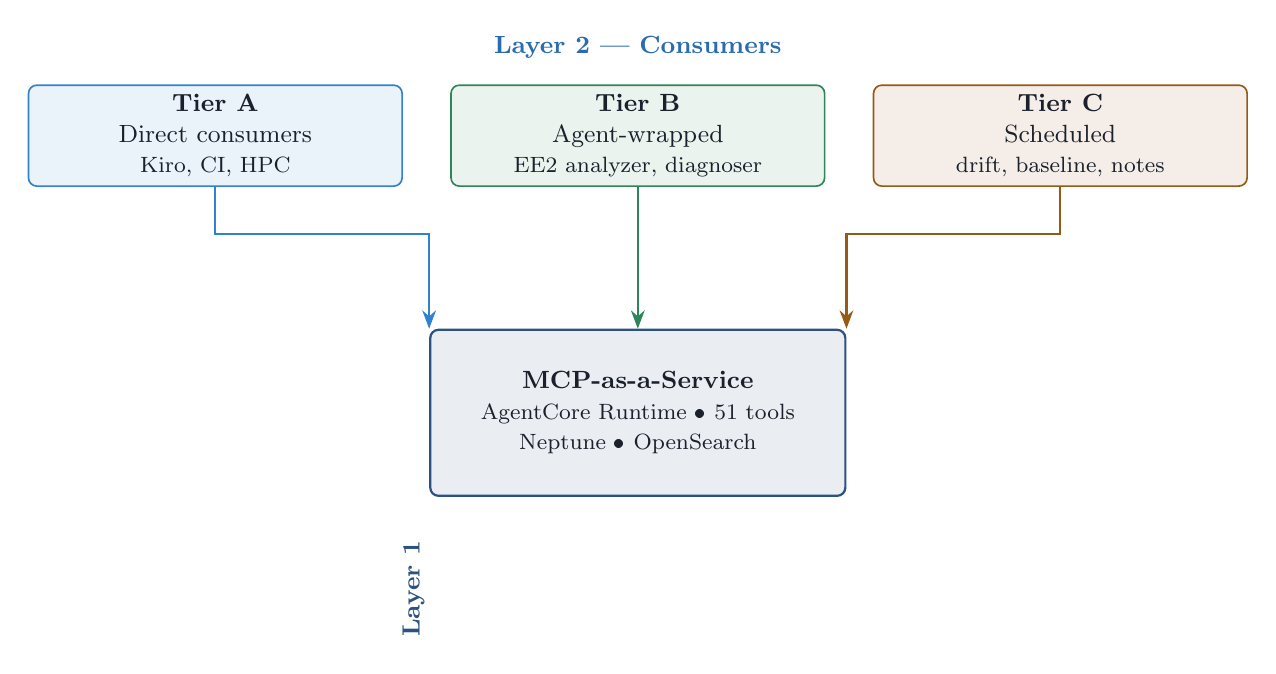
\begin{tikzpicture}[
    node distance=6mm,
    tier/.style={rectangle, rounded corners=3pt, draw=#1, line width=0.6pt,
                 fill=#1!10, text=ink, minimum width=13.5em,
                 minimum height=2.5em, align=center, font=\small},
    label/.style={font=\bfseries\small, text=#1},
    layer1box/.style={rectangle, rounded corners=3pt,
                      draw=layer1, line width=0.8pt, fill=layer1!10,
                      minimum width=15em, minimum height=6em,
                      align=center, font=\small, text=ink},
    arrow/.style={-Stealth, thick, draw=#1}
]

% Layer 2 tiers
\node[tier=layer2a] (ta) at (0,0) {\textbf{Tier A}\\Direct consumers\\{\footnotesize Kiro, CI, HPC}};
\node[tier=layer2b, right=of ta] (tb) {\textbf{Tier B}\\Agent-wrapped\\{\footnotesize EE2 analyzer, diagnoser}};
\node[tier=layer2c, right=of tb] (tc) {\textbf{Tier C}\\Scheduled\\{\footnotesize drift, baseline, notes}};

% Layer label
\node[label=accent, above=2mm of tb] (l2lab) {Layer 2 --- Consumers};

% Layer 1
\node[layer1box, below=18mm of tb] (l1) {\textbf{MCP-as-a-Service}\\{\footnotesize AgentCore Runtime \textbullet\ 51 tools}\\{\footnotesize Neptune \textbullet\ OpenSearch}};
\node[label=layer1, left=2mm of l1, anchor=east, rotate=90, xshift=-15mm] {\small Layer 1};

% Arrows
\draw[arrow=layer2a] (ta.south) -- ++(0,-6mm) -| (l1.north west);
\draw[arrow=layer2b] (tb.south) -- (l1.north);
\draw[arrow=layer2c] (tc.south) -- ++(0,-6mm) -| (l1.north east);

\end{tikzpicture}
\end{center}

\subsubsection*{Tier A --- Direct consumers}

Tier A consumers treat the MCP as their own tool source. They make
individual tool calls and compose results in their own client logic.

\begin{itemize}[leftmargin=*, itemsep=2pt]
  \item \textbf{Kiro IDE} on a developer workstation or laptop.
  \item \textbf{GitHub Actions CI} pipelines performing root-cause
        analysis on failed builds.
  \item \textbf{HPC researcher sessions} on Hera, Orion, Hercules,
        Gaea, or Ursa.
\end{itemize}

\subsubsection*{Tier B --- Agent-wrapped consumers}

Tier B is where the real leverage lives. An agent is a small
AgentCore-hosted service (a fork of the \texttt{HelloAgent} scaffold,
typically 80--150 lines of Python) that uses a foundation model to
orchestrate multiple MCP tool calls into a cohesive analytical
response.

The user sees one endpoint. Behind it, the agent may make a dozen
MCP calls, reason over the results, run code in a sandbox, and
synthesize a final answer.

\begin{itemize}[leftmargin=*, itemsep=2pt]
  \item \textbf{EE2 Compliance Analyzer}: code or logs in, EE2
        diagnosis out, with suggested fixes.
  \item \textbf{Build Failure Diagnoser}: Rocoto failure log in,
        root-cause narrative and recommended fix location out.
  \item \textbf{Code Review Assistant}: PR diff in, EE2-aware and
        change-impact-aware review comments out.
  \item \textbf{Onboarding Docent}: natural-language Q\&A about
        Global Workflow, for new developers and rotating staff.
\end{itemize}

\subsubsection*{Tier C --- Scheduled consumers}

Tier C runs on a cadence rather than on user demand.

\begin{itemize}[leftmargin=*, itemsep=2pt]
  \item Nightly knowledge-base drift monitor.
  \item Weekly EE2 compliance baseline report.
  \item On-tag release notes generator.
\end{itemize}

\begin{impact}
A single upstream change in \texttt{mcp\_server\_node} can reach a
dozen downstream consumers without coordinated redeploys. A new
consumer can be built in a day without any change to the MCP server.
\end{impact}

% ============== Section 3: The architecture diagram ==================
\section{Reference architecture}

Figure~\ref{fig:twolayer} shows the complete system after Phase~B
completes.

\begin{figure}[h]
\centering
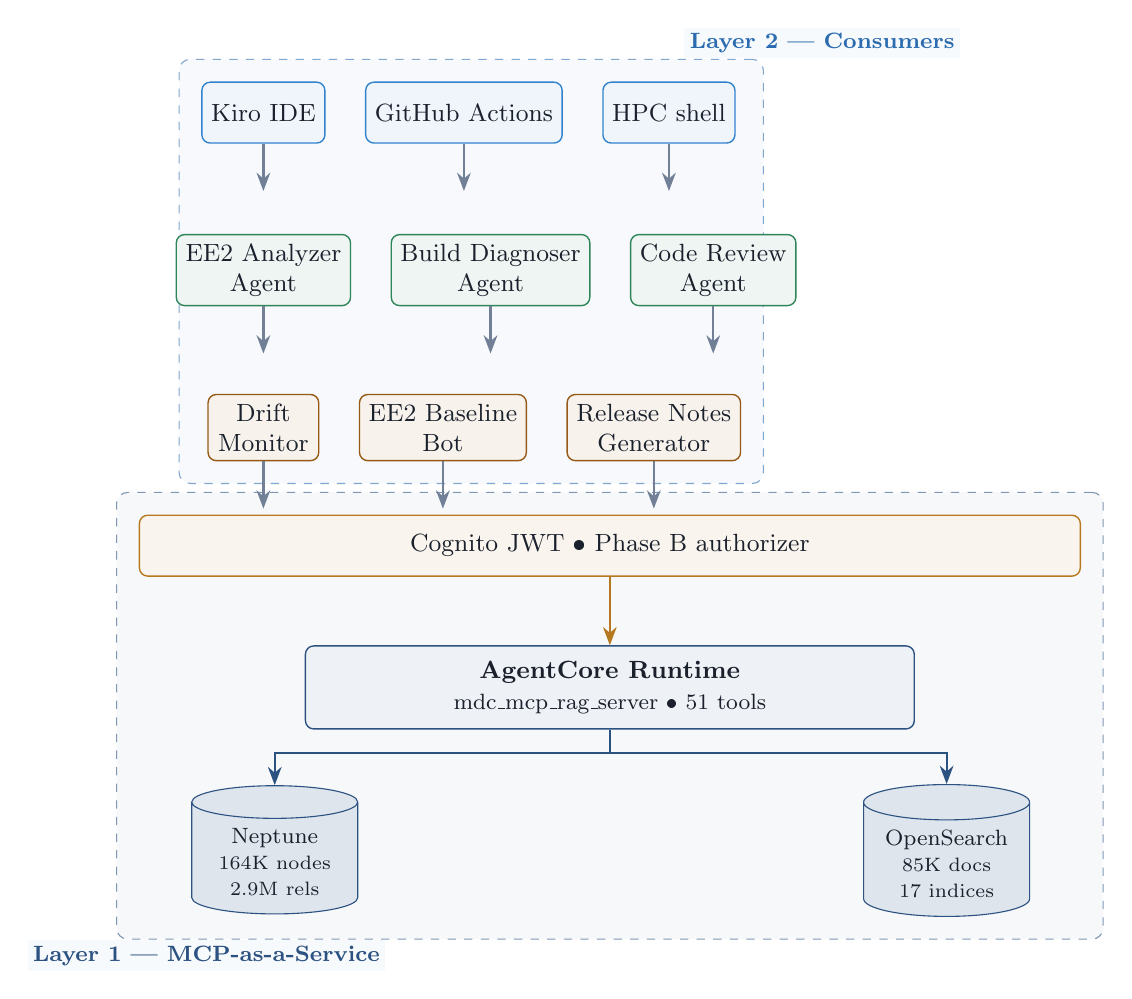
\begin{tikzpicture}[
    font=\small,
    node distance=5mm,
    box/.style={rectangle, rounded corners=3pt, draw=#1,
                line width=0.5pt, fill=#1!8, minimum height=2.2em,
                minimum width=4em, align=center, text=ink},
    datastore/.style={cylinder, shape border rotate=90, aspect=0.25,
                      draw=layer1, fill=layer1!15, minimum height=4em,
                      minimum width=6em, align=center, text=ink,
                      font=\footnotesize},
    arrow/.style={-Stealth, thick, draw=#1},
    layerbox/.style={rectangle, rounded corners=4pt, draw=#1!60,
                     line width=0.4pt, fill=#1!4, dashed},
    layerlabel/.style={text=#1, font=\bfseries\footnotesize,
                       fill=paper, inner sep=2pt}
]

% Tier A consumers (left column of layer 2)
\node[box=layer2a] (kiro) at (0,6) {Kiro IDE};
\node[box=layer2a, right=of kiro] (ci) {GitHub Actions};
\node[box=layer2a, right=of ci] (hpc) {HPC shell};

% Tier B agents (middle of layer 2)
\node[box=layer2b] (a1) at (0,4) {EE2 Analyzer\\Agent};
\node[box=layer2b, right=of a1] (a2) {Build Diagnoser\\Agent};
\node[box=layer2b, right=of a2] (a3) {Code Review\\Agent};

% Tier C (bottom row of layer 2)
\node[box=layer2c] (sc1) at (0,2) {Drift\\Monitor};
\node[box=layer2c, right=of sc1] (sc2) {EE2 Baseline\\Bot};
\node[box=layer2c, right=of sc2] (sc3) {Release Notes\\Generator};

% Auth gateway (Phase B Cognito)
\node[box=emcgold, minimum width=34em] (cog) at (4.4,0.5) {Cognito JWT \textbullet\ Phase B authorizer};

% Layer 1: AgentCore Runtime
\node[box=layer1, minimum width=22em, minimum height=3em] (acr) at (4.4,-1.3)
    {\textbf{AgentCore Runtime}\\{\footnotesize mdc\_mcp\_rag\_server \textbullet\ 51 tools}};

% Data stores
\node[datastore, below left=8mm and -5mm of acr] (neptune)
    {Neptune\\{\scriptsize 164K nodes}\\{\scriptsize 2.9M rels}};
\node[datastore, below right=8mm and -5mm of acr] (os)
    {OpenSearch\\{\scriptsize 85K docs}\\{\scriptsize 17 indices}};

% Arrows: consumers to Cognito / AgentCore
\foreach \src in {kiro, ci, hpc, a1, a2, a3, sc1, sc2, sc3}
    \draw[arrow=subtle, -Stealth] (\src.south) -- ++(0,-6mm);
\draw[arrow=emcgold] (cog.south) -- (acr.north);

% Arrows: runtime to data stores
\draw[arrow=layer1] (acr.south) -- ++(0,-3mm) -| (neptune.north);
\draw[arrow=layer1] (acr.south) -- ++(0,-3mm) -| (os.north);

% Layer 2 background
\begin{scope}[on background layer]
\node[layerbox=accent, fit=(kiro)(sc3),
      inner sep=8pt, label={[layerlabel=accent]above right:Layer 2 --- Consumers}] {};
\node[layerbox=layer1, fit=(cog)(acr)(neptune)(os),
      inner sep=8pt, label={[layerlabel=layer1]below left:Layer 1 --- MCP-as-a-Service}] {};
\end{scope}

\end{tikzpicture}
\caption{The two-layer architecture. Layer~2 consumers of all three tiers
converge on a single Cognito-authenticated AgentCore Runtime endpoint.
Each consumer type carries a distinct principal identity and a
scope-limited tool set. Neptune and OpenSearch remain VPC-private;
the Runtime is the only public surface.}
\label{fig:twolayer}
\end{figure}

% ============== Section 4: Concrete agent use cases ==================
\section{Three use cases that become viable today}

The following three scenarios illustrate how Layer~2 transforms the
developer experience. All three are achievable with current infrastructure
once Phase~B Cognito authorization ships.

\subsection{Use case 1: EE2 compliance on every failed CI build}

When a GitHub Actions build of a contributor's PR fails, a downstream job
automatically assumes a federated IAM role (via GitHub OIDC), exchanges
that identity for a short-lived Cognito JWT, and calls the
\textbf{EE2 Compliance Analyzer Agent}. The agent:

\begin{enumerate}[leftmargin=*, itemsep=1pt]
  \item Receives the failed-build log.
  \item Calls the MCP's \texttt{analyze\_ee2\_compliance} on the modified
        files in the PR.
  \item Calls \texttt{search\_ee2\_standards} and \texttt{search\_documentation}
        for context on any violations found.
  \item Calls \texttt{find\_callers\_callees} to understand the blast
        radius of the violating code.
  \item Synthesizes a structured PR comment with findings, severity,
        references to the EE2 standards, and suggested fixes.
\end{enumerate}

\begin{impact}
Every PR becomes its own compliance review, automatically.
Contributors receive standards-aware guidance in minutes instead of
waiting for human reviewers. EMC reviewers focus on judgment calls
rather than boilerplate compliance checks.
\end{impact}

\subsection{Use case 2: Root-cause analysis on Rocoto failures}

An operations engineer receives a Slack alert for a failed overnight
Rocoto workflow. Instead of opening a terminal on HPC and grep-ing logs,
they paste the workflow name into a chat interface backed by the
\textbf{Build Failure Diagnoser Agent}. The agent:

\begin{enumerate}[leftmargin=*, itemsep=1pt]
  \item Retrieves the job's configuration via
        \texttt{get\_job\_details}.
  \item Traces the execution path via
        \texttt{trace\_execution\_path} and
        \texttt{trace\_full\_execution\_chain}.
  \item Pulls the job's environment variable dependencies via
        \texttt{find\_env\_dependencies}.
  \item Searches documentation for known-issue patterns via
        \texttt{search\_documentation}.
  \item Returns a plain-language narrative: what the job does, which
        step likely failed, why, and where to look in the code.
\end{enumerate}

\begin{impact}
Mean-time-to-diagnosis for workflow failures drops from hours (requiring
SME attention) to minutes (self-service for any operator). The SME is
re-engaged only for novel failures, not repeat patterns.
\end{impact}

\subsection{Use case 3: Natural-language onboarding for new developers}

A new hire starting on the UFS coupled model uses an
\textbf{Onboarding Docent Agent} from their laptop. They ask:
\textit{``Explain how data assimilation feeds into the forecast cycle.''}
The agent:

\begin{enumerate}[leftmargin=*, itemsep=1pt]
  \item Calls \texttt{search\_architecture} for high-level community
        summaries.
  \item Calls \texttt{explain\_with\_context} for technical depth.
  \item Calls \texttt{get\_operational\_guidance} for HPC-specific
        runtime considerations.
  \item Stitches the results into a coherent narrative with citations
        back to documentation and code.
\end{enumerate}

\begin{impact}
Onboarding that historically took weeks of shadowing collapses into
self-service exploration, with senior staff freed to teach the
non-obvious parts. New hires ramp faster; institutional knowledge is
queryable, not tribal.
\end{impact}

% ============== Section 5: Quantitative framing ======================
\section{Why the economics work}

Three independent charts illustrate why the two-layer partition is the
correct engineering bet.

\subsection{Lines of code per capability}

\begin{figure}[h]
\centering
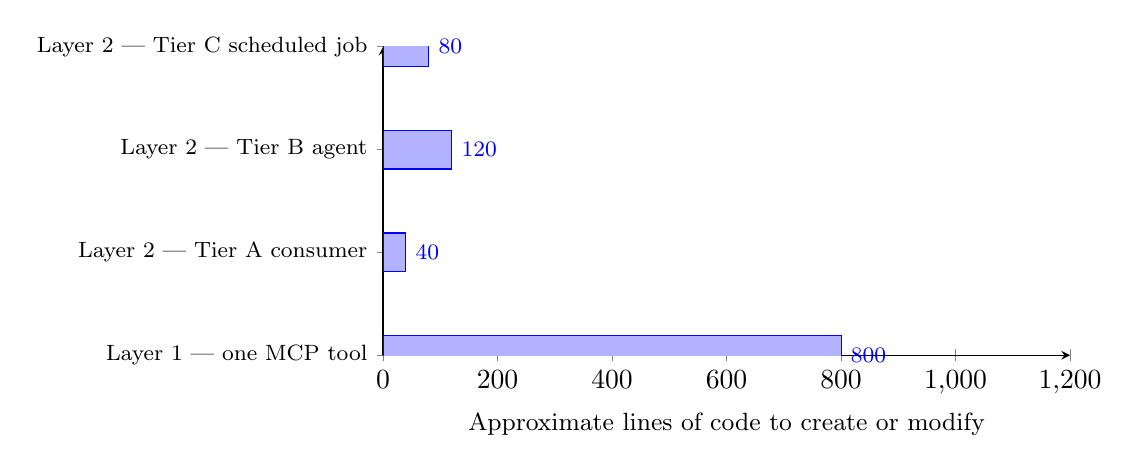
\begin{tikzpicture}
\begin{axis}[
  width=0.85\linewidth, height=5.5cm,
  xbar, bar width=14pt,
  symbolic y coords={L1tool, L2A, L2B, L2C},
  ytick=data,
  yticklabels={Layer 1 --- one MCP tool,
               Layer 2 --- Tier A consumer,
               Layer 2 --- Tier B agent,
               Layer 2 --- Tier C scheduled job},
  xlabel={Approximate lines of code to create or modify},
  nodes near coords, nodes near coords style={font=\footnotesize},
  xmin=0, xmax=1200,
  enlarge y limits=0.15,
  axis lines=left,
  ylabel style={font=\small},
  xlabel style={font=\small},
  y tick label style={font=\footnotesize, align=right},
  every axis plot/.append style={fill=accent!60, draw=accent},
]
\addplot coordinates {(800,L1tool) (40,L2A) (120,L2B) (80,L2C)};
\end{axis}
\end{tikzpicture}
\caption{Adding capability at Layer~2 is roughly an order of magnitude
cheaper than adding it at Layer~1. Layer~1 changes require graph
schema considerations, data access layer integration, and cross-backend
testing; Layer~2 changes are mostly a system prompt plus tool selection.}
\label{fig:loc}
\end{figure}

\subsection{Blast radius on failure}

\begin{figure}[h]
\centering
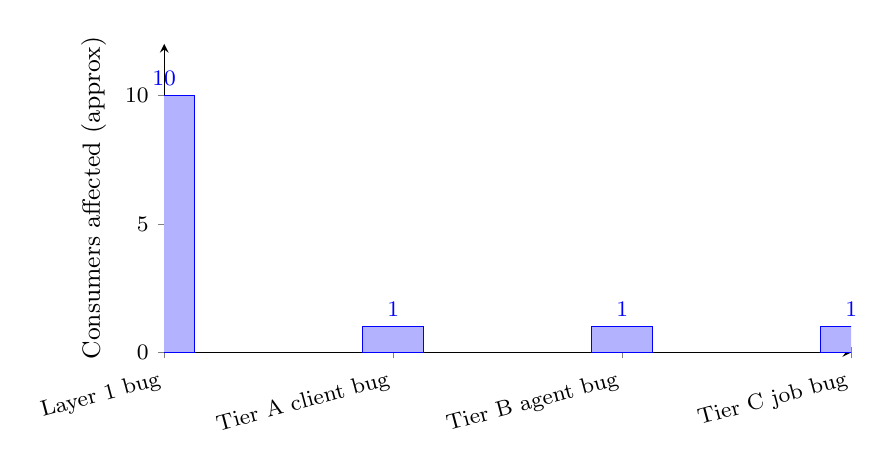
\begin{tikzpicture}
\begin{axis}[
  width=0.85\linewidth, height=5.5cm,
  ybar, bar width=22pt,
  symbolic x coords={L1bug, TAbug, TBbug, TCbug},
  xtick=data,
  xticklabels={Layer 1 bug, Tier A client bug, Tier B agent bug, Tier C job bug},
  ylabel={Consumers affected (approx)},
  nodes near coords, nodes near coords style={font=\footnotesize},
  ymin=0, ymax=12,
  enlarge x limits=0.15,
  axis lines=left,
  ylabel style={font=\small},
  y tick label style={font=\footnotesize},
  x tick label style={font=\footnotesize, rotate=15, anchor=north east},
  every axis plot/.append style={fill=warm!55, draw=warm},
]
\addplot coordinates {(L1bug,10) (TAbug,1) (TBbug,1) (TCbug,1)};
\end{axis}
\end{tikzpicture}
\caption{Failure isolation. A bug in Layer~1 potentially degrades every
consumer; a bug in any single Layer~2 consumer is contained to that
consumer. This is why Layer~1 is kept narrow and stable while Layer~2
can iterate rapidly.}
\label{fig:blastradius}
\end{figure}

\subsection{Where reasoning lives}

\begin{figure}[h]
\centering
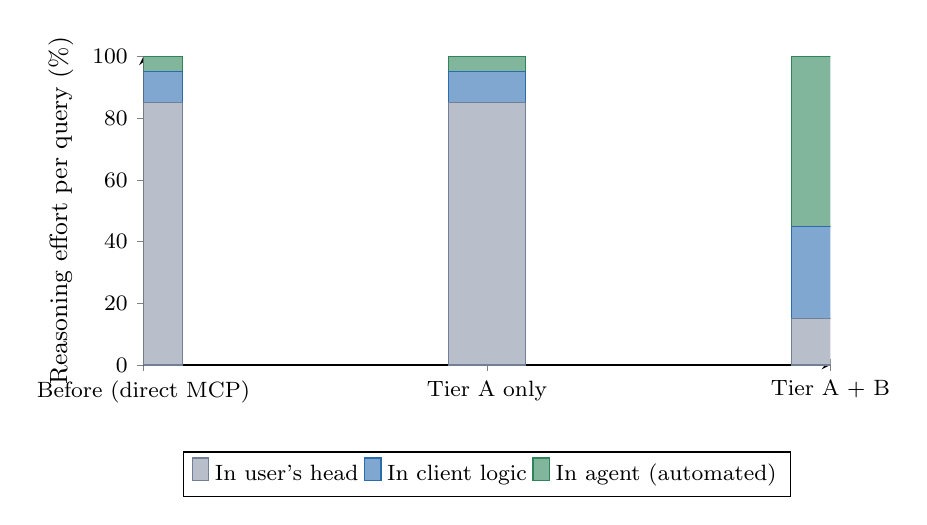
\begin{tikzpicture}
\begin{axis}[
  width=0.85\linewidth, height=5.5cm,
  ybar stacked, bar width=28pt,
  symbolic x coords={Before, TierA, TierAB},
  xtick=data,
  xticklabels={Before (direct MCP), Tier A only, Tier A + B},
  ylabel={Reasoning effort per query (\%)},
  ymin=0, ymax=100,
  enlarge x limits=0.3,
  axis lines=left,
  legend style={at={(0.5,-0.28)}, anchor=north, legend columns=-1, font=\footnotesize},
  x tick label style={font=\footnotesize},
  y tick label style={font=\footnotesize},
  ylabel style={font=\small},
]
\addplot+[fill=subtle!50, draw=subtle] coordinates {(Before,85) (TierA,85) (TierAB,15)};
\addplot+[fill=accent!60, draw=accent] coordinates {(Before,10) (TierA,10) (TierAB,30)};
\addplot+[fill=ok!60, draw=ok] coordinates {(Before,5) (TierA,5) (TierAB,55)};
\legend{In user's head, In client logic, In agent (automated)}
\end{axis}
\end{tikzpicture}
\caption{Cognitive load shift. Without Tier~B agents, the bulk of
orchestration lives in the user's head or is copy-pasted across client
scripts. Tier~B agents push that orchestration into automated,
version-controlled code paths.}
\label{fig:reasoningshift}
\end{figure}

% ============== Section 6: Trust, cost, and governance ===============
\section{Trust, cost, and governance properties}

\subsection{Trust boundaries}

Each Layer~2 consumer has its own identity:

\begin{itemize}[leftmargin=*, itemsep=2pt]
  \item Tier A consumers present a per-call JWT whose \texttt{sub}
        claim identifies the user or CI run.
  \item Tier B agents run under their own AgentCore execution role
        and hold their own Cognito client credentials.
  \item Tier C scheduled jobs run under EventBridge-invoked IAM
        roles, again distinct from any other consumer.
\end{itemize}

\noindent
A compromise or misbehavior of any single consumer is contained. Revoking
its Cognito client disables it without touching the MCP server or other
consumers. This is a substantial improvement over a monolithic agent that
holds privileges for all downstream interactions.

\subsection{Cost attribution}

AgentCore bills per runtime session. Because each agent is its own
runtime, AWS cost explorer naturally attributes spend to each agent by
name. The MCP server's cost is attributable separately. Leadership can
see, line-by-line, which analytical capabilities are consuming budget
and make informed decisions about where to invest.

\subsection{Model flexibility}

Foundation model choice is an agent-by-agent decision. A compliance
auditor might justify Claude Sonnet for quality; a batch-mode release
notes generator might pick Claude Haiku for cost; a niche agent might
try Nova. The MCP server is model-agnostic---it exposes tool schemas
and returns structured results---so no Layer~1 change is ever required
to try a new model at Layer~2.

\subsection{Governance}

EE2 compliance standards themselves live in the knowledge base
(\texttt{search\_ee2\_standards}, \texttt{analyze\_ee2\_compliance}).
Every agent that analyzes code against standards is using the same
authoritative reference. When standards evolve, all agents see the
update immediately---no agent-side code change is needed. This is the
consequence of Layer~1 being the single source of analytical truth.

% ============== Section 7: What this means for EMC ===================
\section{What this means for EMC}

\begin{mdframed}[linecolor=ok, linewidth=0.8pt, backgroundcolor=paper,
                  leftmargin=0pt, rightmargin=0pt, innertopmargin=10pt,
                  innerbottommargin=10pt, innerleftmargin=12pt,
                  innerrightmargin=12pt, roundcorner=3pt]
The deployment of the MDC MCP RAG Server to AWS Bedrock AgentCore is not
the end of a project. It is the \emph{platform enablement} step for a
family of analytical assistants that live close to the work---in CI
pipelines, on HPC login nodes, in chat interfaces, on developer
laptops---each focused on a single job, each independently evolvable,
each drawing on a shared institutional knowledge base.

Three things become possible this quarter:

\begin{enumerate}[leftmargin=*, itemsep=2pt]
  \item \textbf{Automatic EE2 review on every CI build}, reducing
        reviewer load and compressing contributor feedback cycles.
  \item \textbf{Self-service root-cause analysis} for workflow failures,
        reclaiming SME time and shortening mean-time-to-diagnosis.
  \item \textbf{Natural-language onboarding} for new developers and
        rotating staff, accelerating ramp and preserving institutional
        knowledge as queryable context.
\end{enumerate}

None of these require invention. They require building on what is now
a production-ready platform.
\end{mdframed}

% ============== Section 8: Roadmap signposts =========================
\section{Roadmap signposts}

The Phase~B external-access spec (\texttt{.kiro/specs/mcp-external-access/})
delivers the plumbing: Cognito authentication, GitHub Actions OIDC
federation, HPC command-line helper, per-principal tool scoping, and
audit logging. Completion is expected in Q2~2026.

After Phase~B, the natural next projects are the Tier~B agents described
in Section~4. The \texttt{HelloAgent/} scaffold in the repository---an
AWS-provided template---is an $\sim$80-line reference implementation
showing exactly how such an agent is structured. Each production agent
will be a purpose-specific fork of that scaffold.

Phase~C (AgentCore Gateway with Cedar tool-level policies) is deferred
and addresses a future scaling concern: fine-grained per-tool
authorization and centralized audit enrichment. It is not needed for
the use cases described in this paper.

\vspace{8pt}
\hrule
\vspace{8pt}
\footnotesize
\textit{Prepared by the MDC MCP RAG team. For questions, technical
detail, or code walkthroughs of the HelloAgent scaffold, contact the
team via the EMC MCP-access channel.}

\end{document}
